\section{开发环境}\label{sec:DevelopmentEnvironment}

在本节(\cref{sec:DevelopmentEnvironment})中,笔者将详细介绍 MinmusOS 项目的开发环境,包括使用的操作系统(Windows 11)、开发工具(Windows Subsystem for Linux、Ubuntu 22.04 LTS、QEMU 模拟器、JetBrains RustRover、Rust 语言),并深入讲解开发环境的搭建过程、项目配置及自动化构建的设置。最后,笔者还将介绍如何在配置好的环境中运行 MinmusOS 项目,以确保开发者能够顺利进行开发和调试。

\subsection{开发环境概述}

本项目的开发环境如下:

\begin{enumerate}
    \item 开发环境
          \begin{enumerate}
              \item Windows 11 家庭中文版 23H2
              \item Windows Subsystem for Linux (WSL) 2.2.4.0
              \item Ubuntu 22.04.3 LTS
              \item QEMU 模拟机(qemu-system-i386)6.2.0
          \end{enumerate}
    \item 开发软件
          \begin{enumerate}
              \item JetBrains RustRover 2024.1.7
          \end{enumerate}
    \item 开发语言
          \begin{enumerate}
              \item Rust 语言(Rustup:1.27.1,Rustc:1.82.0-nightly,Cargo:1.82.0-nightly)
          \end{enumerate}
\end{enumerate}

\subsubsection{Windows 11}

使用Windows系统来开发操作系统内核,尽管可能不如Linux环境那样常见,但仍然有其独特的优势和便利性。以下是使用Windows系统开发操作系统内核的几个主要优势:

\begin{enumerate}
    \item \textbf{熟悉的开发环境}:对于习惯使用Windows的开发者来说,继续在这个环境下工作可以减少学习新工具和操作系统的时间,使他们能够更专注于开发工作本身。Windows的用户界面、文件系统管理、任务管理等都是开发者熟悉的。
    \item \textbf{强大的开发工具}:Windows支持多种强大的开发环境,如Visual Studio Code。这些IDE提供了先进的代码编辑、项目管理、版本控制和调试工具。
    \item \textbf{使用WSL提升开发效率}:通过集成了WSL(Windows Subsystem for Linux),Windows环境可以无缝地运行Linux工具和软件,结合了Linux的命令行工具和Windows的图形界面优势。这允许开发者在不离开Windows的情况下使用Linux环境,例如使用GCC、Make、GDB等工具进行内核开发。
    \item \textbf{文档和社区资源}:Windows拥有庞大的开发者社区和丰富的文档资源,对于解决开发中的问题和学习新技术都极为有用。
\end{enumerate}

总体而言,虽然Linux通常是内核开发的首选环境,但Windows提供的工具、支持和兼容性使其成为许多情况下一个可行且有效的选择,尤其是结合了WSL后,Windows在操作系统内核开发方面的适用性大大提高。

\subsubsection{Windows Subsystem for Linux (WSL)}

使用 Windows Subsystem for Linux (WSL) 在开发操作系统内核时具有一系列优势,特别是对于习惯使用Windows环境的开发者来说。这些优势包括:

\begin{enumerate}
    \item \textbf{集成Windows和Linux环境}:WSL允许开发者在Windows系统上运行Linux环境,无需重启进入另一个操作系统或使用虚拟机。这意味着可以利用Windows的图形界面和生产力工具(如VSCode),同时执行Linux命令行工具和应用。
    \item \textbf{简化开发流程}:对于需要同时访问Windows和Linux工具的开发任务,WSL提供了极大的便利。开发者可以在相同的文件系统中访问项目文件,使用Windows编辑器编辑代码,然后在Linux环境中编译和测试,无需文件转移或复制。
    \item \textbf{资源占用更少}:与传统的虚拟机相比,WSL提供了更轻量级的解决方案。它直接在Windows内核上运行,减少了资源占用,启动和运行速度更快,对系统性能的影响也更小。
    \item \textbf{方便的环境管理}:WSL允许开发者安装多个Linux发行版,可以在不同的项目或任务之间切换不同的环境。例如,可以在一个发行版上进行开发工作,而在另一个发行版上进行测试。
    \item \textbf{直接访问硬件和系统调用}:WSL使用真实的Linux内核,这使得它在处理系统调用和操作硬件时表现得更接近传统Linux系统。这对于需要进行底层系统开发的项目尤其重要,因为它允许开发者在接近生产环境的条件下测试和开发。
    \item \textbf{持续集成和交叉编译支持}:使用WSL,开发者可以在同一机器上进行交叉编译,为不同的平台构建应用程序,包括Linux、Windows和其他操作系统。这种能力对于开发涉及多平台支持的内核或应用程序非常有用。
    \item \textbf{社区和官方支持}:Microsoft对WSL的持续更新和支持确保了其与现代硬件和软件技术的兼容性。此外,广泛的开发者社区也提供了大量的教程、工具和第三方应用支持,这对于解决开发中的问题非常有帮助。
\end{enumerate}

WSL是为那些想要在Windows系统上利用Linux开发工具的开发者提供了一种非常实用的解决方案,它结合了两个系统的优点,提高了开发效率和灵活性。

\subsubsection{Ubuntu 22.04 LTS}

使用Ubuntu作为开发环境,尤其是在开发操作系统内核这类底层项目时,有几个显著的优势:

\begin{enumerate}
    \item \textbf{稳定性和长期支持}:Ubuntu 22.04 LTS(Long Term Support,长期支持)版本提供了长达五年的安全更新和维护。这意味着开发者可以在一个稳定且长期受支持的平台上工作,无需担心频繁更换操作系统或缺乏安全更新。
    \item \textbf{与生产环境一致}:在Ubuntu上开发可以确保软件在生产环境中运行时表现得更加可靠和高效,因为开发和生产环境可以保持高度一致。
    \item \textbf{广泛的社区支持和资源}:Ubuntu拥有庞大的用户和开发者社区,这意味着大量的文档、论坛和支持资源可供查阅。这对于解决开发中遇到的问题非常有帮助。
    \item \textbf{开源工具和库的兼容性}:Ubuntu提供了丰富的开源开发工具和库。对于操作系统开发而言,这些工具(如GCC、Make、GDB)都是不可或缺的,而且通常在Linux系统上的兼容性和性能都非常好。
    \item \textbf{适合底层开发}:Linux系统提供了丰富的底层系统调用和接口,这对于内核开发是非常重要的。开发者可以直接与硬件和底层系统资源交互,更方便地实现和测试内核级功能。
    \item \textbf{环境一致性和隔离性}:使用容器和虚拟化技术(如Docker和QEMU),可以在Ubuntu上轻松创建和管理隔离的开发环境。这对于测试不同的配置和开发环境至关重要。
\end{enumerate}

总之,选择Ubuntu作为开发环境,可以为操作系统内核的开发提供一个稳定、高效、兼容性好的基础,同时也利于将来在类似环境中部署和运行。

\subsubsection{QEMU 模拟机(qemu-system-i386)}

QEMU是一个功能强大的开源机器模拟器和虚拟化解决方案,对于操作系统内核的开发尤为重要。以下是使用QEMU的一些主要优势:

\begin{enumerate}
    \item \textbf{多平台支持}:QEMU能够模拟多种处理器架构,包括x86、ARM、PowerPC、SPARC、和MIPS等。这意味着开发者可以在一个平台上开发和测试为其他平台设计的内核和应用程序,非常适合交叉平台开发。
    \item \textbf{环境隔离}:使用QEMU进行开发可以确保测试环境与主机操作系统隔离。这种隔离可以防止潜在的软件错误影响到主机系统,特别是在开发涉及底层硬件交互的系统软件时。
    \item \textbf{无需实际硬件}:QEMU允许开发者在没有物理目标硬件的情况下进行开发和测试。这不仅降低了成本,还可以在硬件到达前开始开发工作,加速开发周期。
    \item \textbf{调试支持}:QEMU与各种调试工具(如GDB)集成,可以进行详细的步进执行和调试。这对于操作系统内核开发尤为重要,因为它允许开发者在内核运行时进行观察和修改。
    \item \textbf{快照和即时状态保存}:QEMU支持保存和恢复虚拟机的状态(称为快照)。这使得开发者可以快速回滚到一个已知的良好状态,并从那里重新开始测试,极大地提高了测试的效率。
    \item \textbf{网络模拟}:QEMU还能模拟网络环境,允许开发者测试内核的网络功能,如协议栈和驱动程序,而无需实际的网络硬件。
    \item \textbf{性能和资源利用}:虽然QEMU为功能丰富性提供了强大的支持,但它在性能上的优化也非常有效。QEMU的用户模式模拟可以运行应用程序和驱动程序,而不必模拟整个操作系统,从而减少资源消耗。
    \item \textbf{版本更新和社区支持}:QEMU持续更新和改进,提供了最新的功能和改进,确保开发者可以利用最新的技术进行开发。同时,QEMU的广泛用户和开发者社区提供了丰富的文档、工具和支持。
\end{enumerate}

总体来说,QEMU提供了一个强大、灵活、成本效益高的平台,用于开发、测试和调试操作系统内核和其他系统级软件,特别是在多架构和虚拟化环境中。这使得它成为操作系统开发者的重要工具。

\subsubsection{JetBrains RustRover}

JetBrains的RustRover是一款专门为Rust语言设计的集成开发环境(IDE),其提供了许多功能来支持Rust开发,特别是在开发操作系统内核这类复杂项目时。在使用RustRover开发操作系统内核时,具有如下优势:

\begin{enumerate}
    \item \textbf{代码编辑与分析}:RustRover提供了强大的代码编辑器,支持代码高亮、自动格式化、智能补全等功能,能够极大地提高代码编写的效率。它具备深度的代码分析功能,可以帮助开发者快速定位到潜在的代码问题,比如生命周期错误、类型不匹配等常见于Rust开发中的问题。
    \item \textbf{高级调试工具}:RustRover集成了强大的调试器,支持条件断点、表达式求值、变量观察等功能,这对于操作系统内核的调试至关重要。支持对内存布局、堆栈跟踪等低级特性进行检查,这对于底层系统编程尤其有用。
    \item \textbf{跨平台支持和远程开发}:RustRover支持跨平台开发,可以在Windows、Linux或macOS上进行Rust开发。它还支持远程开发功能,允许开发者在远程服务器上直接编写代码、编译和调试,这对于操作系统开发尤其重要,因为操作系统常常需要在特定硬件或仿真环境(如QEMU)中运行和测试。
    \item \textbf{版本控制集成}:RustRover提供了与Git等版本控制系统的无缝集成,这使得管理大型项目的源代码变得更为方便。
    \item \textbf{项目和构建管理}:该IDE提供了对Cargo的完整支持,包括依赖管理、构建配置和测试,并可以直接从IDE中运行构建脚本和测试,极大地简化了构建过程。
    \item \textbf{社区和插件}:JetBrains拥有活跃的开发者社区,可以轻松找到大量有用的插件和资源,以扩展IDE的功能并适应特定开发需求。
\end{enumerate}

总的来说,RustRover为Rust操作系统内核开发提供了一套完整的工具和功能,使开发更加高效和专业。其强大的代码分析和调试功能,以及便捷的远程开发支持,是开发高性能和低级系统软件的理想选择。

\subsubsection{Rust 语言}

Rust是一门现代的系统编程语言,专为提供高性能与内存安全而设计。Rust具有如下特点:

\begin{enumerate}
    \item \textbf{语言设计和安全性特点}:Rust的目标是允许开发者构建高效且可靠的系统级软件,同时通过语言层面的约束,消除传统语言(如C和C++)中常见的内存错误。Rust的独特之处在于其所有权模型,该模型通过精确控制资源(如内存)的所有权、借用规则和生命周期管理,确保在编译时就消除数据竞争和内存泄漏等问题。
    \item \textbf{内存管理机制}:Rust通过其所有权和借用系统实现了编译期内存安全。每个值在Rust中有一个称为其“所有者”的变量,且同一时间内只能有一个所有者。当所有者超出作用域时,值和其占用的内存会被自动清理。此外,Rust通过借用规则(可变借用和不可变借用),允许程序在保证安全性的同时访问数据,而不产生运行时开销。这些特性使Rust能够在不使用垃圾收集的情况下,有效管理内存,避免传统编程语言中常见的内存安全问题。
    \item \textbf{类型系统和数据抽象}:Rust拥有一个表达能力强大的类型系统和类型推断功能,支持泛型、特征(traits)和生命周期(lifetimes)。这些特性允许Rust程序表达高层次的抽象而不牺牲性能。例如,特征可以用来定义共享的行为,泛型则允许在不同类型之间重用代码,而生命周期则确保引用的有效性,防止悬垂引用等问题。这样的类型系统增强了代码的安全性和维护性,使得复杂的系统设计更加简洁和健壮。
    \item \textbf{并发编程的支持}:Rust的设计从一开始就考虑到并发,其所有权和借用机制自然地避免了数据竞争。Rust提供了多种并发编程模型,包括使用消息传递来交换数据、共享状态的线程安全智能指针等。这些机制都是在编译时进行安全检查的,确保并发操作的安全性,大大简化了并发系统的开发和维护。
    \item \textbf{错误处理和异常管理}:Rust采用\texttt{Result<T, E>}和\texttt{Option<T>}类型来显式处理可能的错误和不存在的值,这与C语言中常见的隐式错误代码或异常处理不同。这种方法鼓励开发者前置处理所有潜在的错误情况,从而增加代码的可靠性。此外,Rust也支持通过panic!宏处理不可恢复的错误,当系统遇到严重错误时立即终止执行,这类似于其他语言的异常抛出机制。
\end{enumerate}

通过这些现代的语言特性,Rust提供了一个更安全、更可控的环境,适合开发需要高度可靠性和性能的操作系统内核。这使Rust成为一个对于系统级编程尤为有利的选择。

对于C/C++语言在操作系统开发中的传统地位、C/C++语言在操作系统开发中的劣势以及Rust语言在操作系统开发中的优势在\cref{sec:SystemTechnicalSelection}中有详细阐述。

\subsection{开发环境搭建}

\subsubsection{配置Windows Subsystem for Linux (WSL)}

WSL是一个在Windows操作系统上运行Linux环境的兼容层,允许用户直接在Windows中安装和使用Linux环境。

配置Windows Subsystem for Linux (WSL)的步骤如下:

\begin{enumerate}
    \item 在Visual Studio Code官网下载并安装Visual Studio Code,如\cref{fig:VSCodeWebsite}。
          \begin{figure}[htbp]
              \centering
              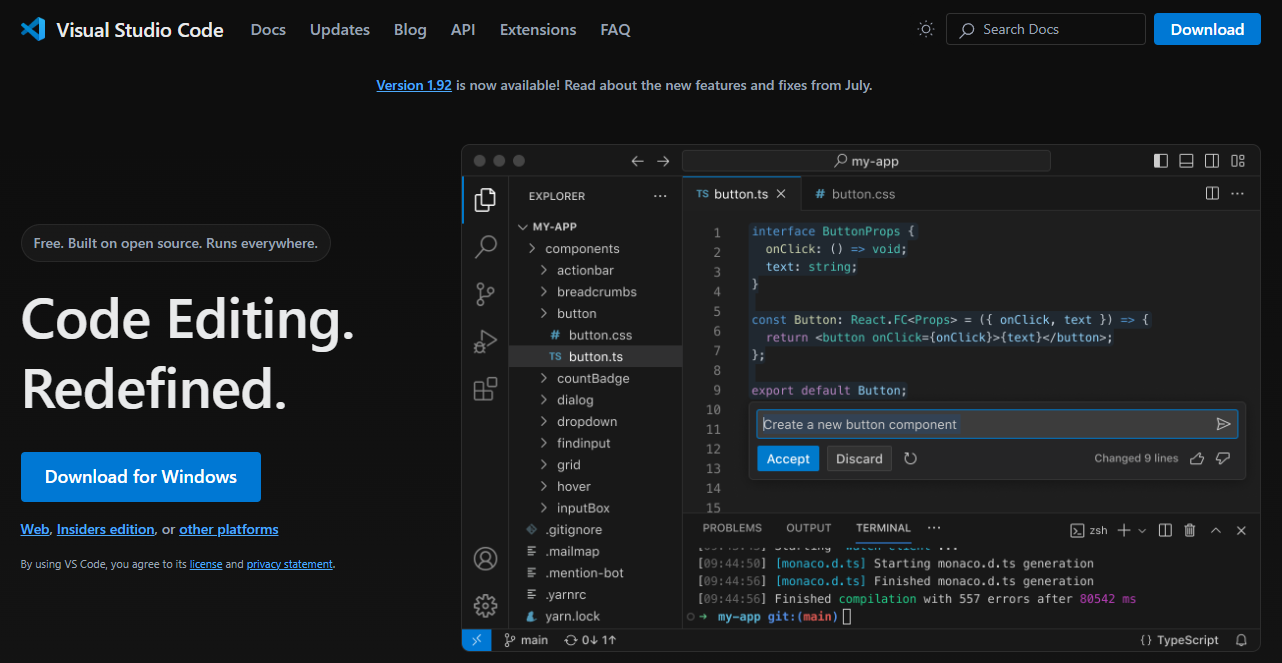
\includegraphics[width=0.8\textwidth]{figures/VSCodeWebsite.png}
              \caption{Visual Studio Code官网}
              \label{fig:VSCodeWebsite}
          \end{figure}
    \item 在Visual Studio Code中向本地安装扩展:WSL,以允许用户在Windows中使用Linux环境,如\cref{fig:ConfigureWSL}。
          \begin{figure}[htbp]
              \centering
              
\includegraphics[width=0.8\textwidth]{figures/ConfigureWSL.png}
              \caption{安装WSL扩展}
              \label{fig:ConfigureWSL}
          \end{figure}
    \item 在“控制面板”>“程序”>“程序和功能”>“启用或关闭Windows功能”中,确定“适用于Linux的Windows子系统”已被选中。
    \item 在“Windows任务管理器”>“性能”>“CPU”选项卡中,确定“虚拟化”已启用。
    \item 启动Windows PowerShell,执行命令\texttt{wsl --version},以查看WSL版本,命令执行结果如\cref{fig:WSLVersion},以验证安装成功。
          \begin{figure}[htbp]
              \centering
              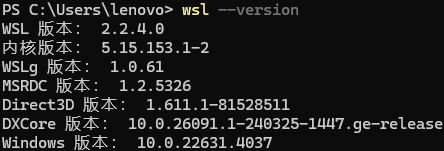
\includegraphics[width=0.6\textwidth]{figures/WSLVersion.png}
              \caption{WSL版本信息}
              \label{fig:WSLVersion}
          \end{figure}
\end{enumerate}

\subsubsection{配置Ubuntu 22.04 LTS}

Ubuntu 22.04 LTS可以为操作系统内核的开发提供一个稳定、高效、兼容性好的基础,同时也利于将来在类似环境中部署和运行。

下面是配置Ubuntu 22.04 LTS的步骤:

\begin{enumerate}
    \item 启动Windows PowerShell,执行命令\texttt{wsl --install Ubuntu-22.04},以安装Ubuntu 22.04 LTS版本到WSL,命令执行结果如\cref{fig:ConfigureUbuntu}。
    \item 在Ubuntu中执行命令\texttt{lsb\_release -a},以查看Linux发行版的详细信息,命令执行结果如\cref{fig:UbuntuVersion},以验证安装成功。
\end{enumerate}

\begin{figure}[htbp]
    \centering
    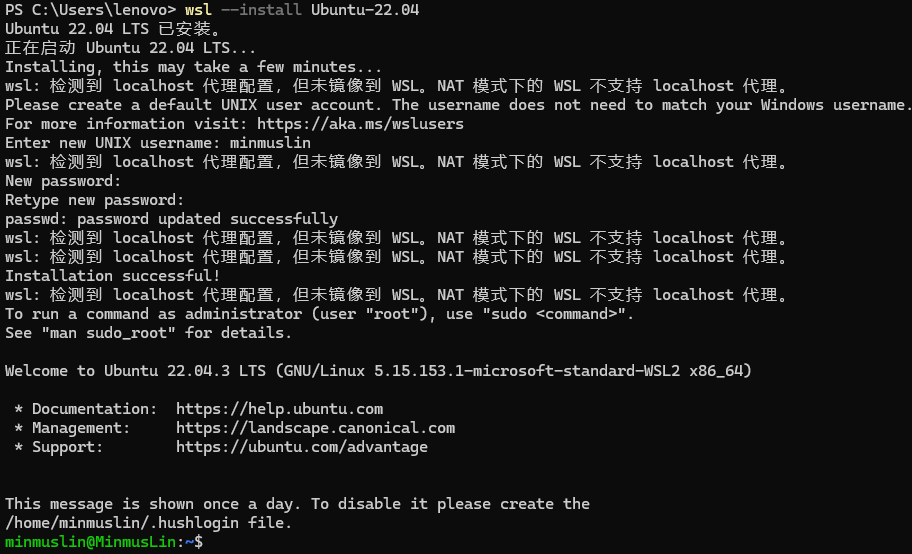
\includegraphics[width=0.8\textwidth]{figures/ConfigureUbuntu.png}
    \caption{配置Ubuntu 22.04 LTS}
    \label{fig:ConfigureUbuntu}
\end{figure}

\begin{figure}[htbp]
    \centering
    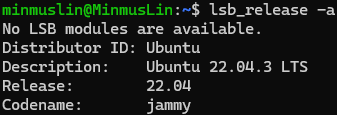
\includegraphics[width=0.6\textwidth]{figures/UbuntuVersion.png}
    \caption{Ubuntu版本信息}
    \label{fig:UbuntuVersion}
\end{figure}

\subsubsection{配置Rust语言开发环境}

Rust是一种注重安全、并发和性能的系统编程语言,旨在帮助开发者构建可靠和高效的软件。RustRover是JetBrains开发的针对于Rust编程语言的集成开发环境(IDE),对Rust语言开发提供了良好的支持。

配置Rust语言开发环境的步骤如下:

\begin{enumerate}
    \item 在JetBrains官网下载并安装JetBrains RustRover,如\cref{fig:RustRoverWebsite}。
          \begin{figure}[htbp]
              \centering
              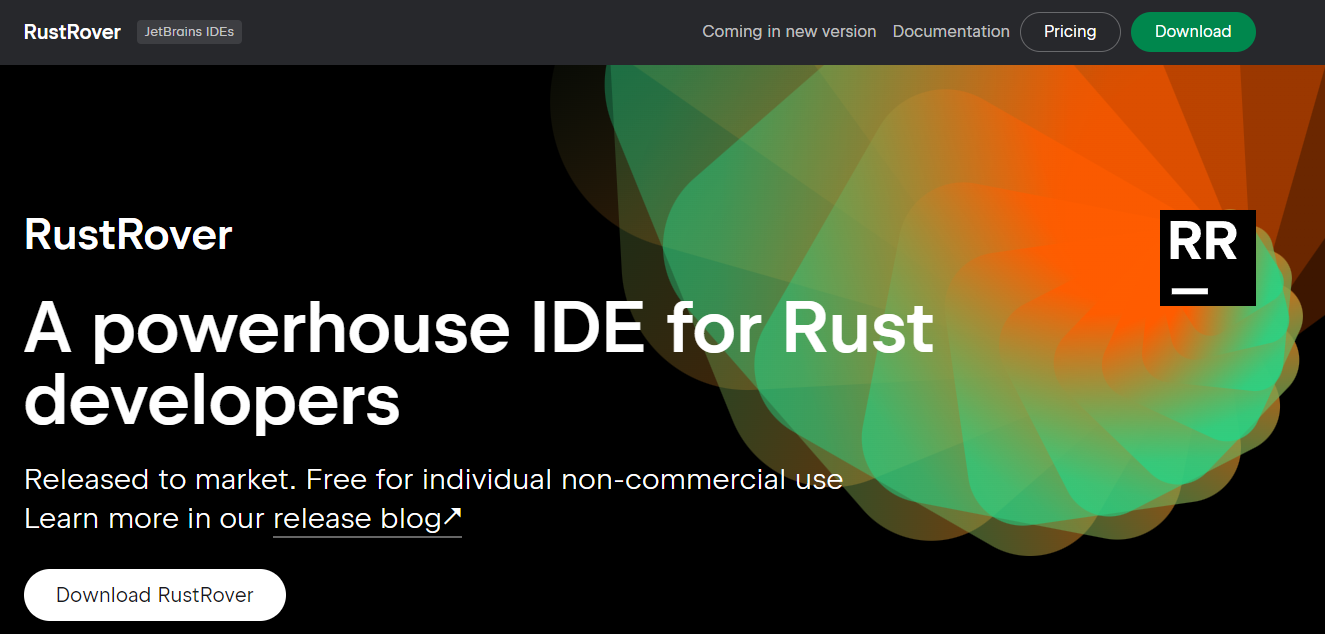
\includegraphics[width=0.8\textwidth]{figures/RustRoverWebsite.png}
              \caption{JetBrains官网}
              \label{fig:RustRoverWebsite}
          \end{figure}
    \item 启动RustRover,在“文件”>“远程开发”>“连接到WSL”中,选择WSL实例为“Ubuntu-22.04”,点击“下一页”。
    \item 在“选择IDE和项目”中,选择IDE版本为“RustRover 2024.1.7 (241.18034.106) | 下载最新”,选择项目目录为“/home/minmuslin/MinmusOS”,如\cref{fig:ConfigureRemoteDevelopment},点击“下载IDE并连接”。
          \begin{figure}[htbp]
              \centering
              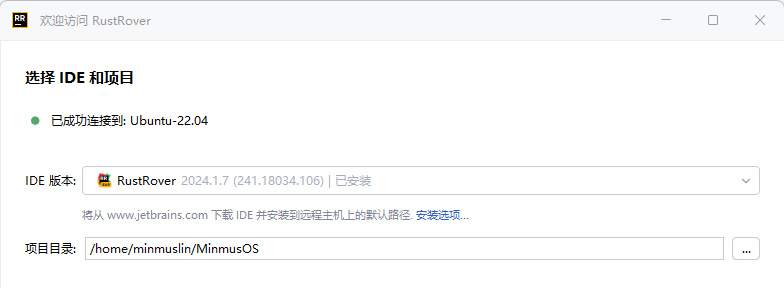
\includegraphics[width=0.8\textwidth]{figures/ConfigureRemoteDevelopment.png}
              \caption{配置远程开发}
              \label{fig:ConfigureRemoteDevelopment}
          \end{figure}
    \item 在“文件”>“设置”>“插件(主机)”中,安装插件“Chinese (Simplified) Language Pack / 中文语言版”和“Makefile Language”,如\cref{fig:RustRoverPlugins}。
          \begin{figure}[htbp]
              \centering
              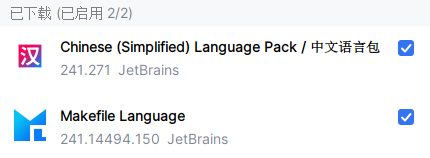
\includegraphics[width=0.6\textwidth]{figures/RustRoverPlugins.png}
              \caption{安装RustRover插件}
              \label{fig:RustRoverPlugins}
          \end{figure}
    \item 新建终端,执行\cref{lst:ConfigureRust},以配置Rust工具链,代码执行结果如\cref{fig:RustVersion},以验证安装成功。每行代码的作用如下:
          \begin{enumerate}
              \item \texttt{curl --proto '=https' --tlsv1.2 -sSf https://sh.rustup.rs | sh}:这行代码通过curl命令从指定的URL下载Rust安装脚本,并通过管道(|)将其传递给sh(Shell)来执行。选项--proto '=https'确保使用HTTPS协议,--tlsv1.2指定使用TLSv1.2版本进行安全连接,-sSf是几个选项的组合,-s表示静默模式,-S表示错误时显示错误,-f表示失败时不显示HTTP错误。
              \item \texttt{source \$HOME/.cargo/env}:执行这行代码会加载Rust的环境配置文件,该文件通常由rustup安装程序在安装Rust时创建于\$HOME/.cargo目录下。source命令用于执行该文件中的命令,以便在当前会话中设置环境变量,使得Rust工具链(如rustc、cargo)可以直接在命令行中使用。
              \item \texttt{rustup update}:这条命令用于更新Rust工具链到最新版本。rustup是Rust的版本管理和安装工具,可以用来管理不同的Rust版本和相关工具。
              \item \texttt{rustup default nightly}:设置Rust的默认工作版本为“nightly”版本。Rust有几个发布频道:stable、beta和nightly。nightly频道提供最新的功能,但可能不够稳定。这行命令将nightly频道设置为默认的Rust版本。
              \item \texttt{rustup --version}:显示当前安装的rustup工具的版本信息。这对于确认rustup是否成功安装及其版本非常有用。
              \item \texttt{rustup --version}:显示Rust编译器(rustc)的版本信息。这用于确认Rust编译器已经安装并可用,同时显示当前编译器的版本。
              \item \texttt{cargo --version}:显示Rust的包管理器和构建工具(cargo)的版本信息。Cargo用于Rust项目的依赖管理和构建,这行命令确认Cargo的安装状态及其版本。
          \end{enumerate}
          \begin{listing}[htbp]
              \begin{minted}{bash}
curl --proto '=https' --tlsv1.2 -sSf https://sh.rustup.rs | sh
source $HOME/.cargo/env
rustup update
rustup default nightly
rustup --version
rustc --version
cargo --version
              \end{minted}
              \caption{配置Rust工具链}\label{lst:ConfigureRust}
          \end{listing}
          \begin{figure}[htbp]
              \centering
              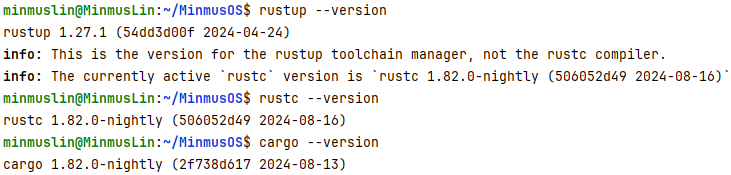
\includegraphics[width=0.8\textwidth]{figures/RustVersion.png}
              \caption{Rust版本信息}
              \label{fig:RustVersion}
          \end{figure}
\end{enumerate}

\subsubsection{配置编译环境与QEMU模拟机(qemu-system-i386)}

在Ubuntu系统配置编译环境的过程中,需要安装一系列的基本工具和库,以支持软件的编译和构建。执行命令\texttt{sudo apt update \&\& sudo apt install build-essential mtools dosfstools fdisk qemu-system-x86}以配置编译环境与QEMU模拟机(qemu-system-i386)。

每个安装的包的作用如下:

\begin{enumerate}
    \item \texttt{build-essential}:这是一个包含编译软件所需的基本编译工具(如gcc编译器、make工具等)的元包。
    \item \texttt{mtools}:一套用来访问MS-DOS磁盘和文件系统的工具,这在处理与DOS或Windows系统相关的磁盘映像时非常有用。
    \item \texttt{dosfstools}:包含用于创建和验证MS-DOS FAT文件系统在Unix和类Unix系统上的磁盘的工具,如mkfs.vfat工具。
    \item \texttt{fdisk}:一个磁盘分区表操作工具,用于创建和修改磁盘分区。
    \item \texttt{qemu-system-x86}:qemu-system-x86是QEMU(Quick Emulator)项目的一部分,它是一个功能强大的开源模拟器和虚拟化工具。特别地,qemu-system-x86是用于模拟x86和x86\_64(也称为AMD64)架构计算机的程序。这使得开发者和测试者可以在不同的操作系统和硬件配置上模拟和运行软件,而无需物理硬件。
\end{enumerate}

\subsection{MinmusOS项目配置}

\subsubsection{项目工作空间和编译选项配置}

\begin{listing}[htbp]
    \begin{minted}{toml}
[unstable]
build-std = ["core", "compiler_builtins", "alloc"]
build-std-features = ["compiler-builtins-mem"]
    \end{minted}
    \caption{.cargo/config.toml配置文件}\label{lst:ConfigToml}
\end{listing}

配置文件.cargo/config.toml(\cref{lst:ConfigToml})的作用如下:

\begin{enumerate}
    \item \texttt{build-std}:这个选项用于指定需要构建的标准库部分。在嵌入式开发或操作系统开发中,通常没有完整的标准库支持,所以需要指定要构建哪些核心库。
          \begin{enumerate}
              \item \texttt{core}:提供基础的Rust功能,适用于没有操作系统支持的环境。
              \item \texttt{compiler\_builtins}:提供编译器相关的内建函数,这在没有标准库的情况下非常重要。
              \item \texttt{alloc}:提供内存分配支持,但不依赖全局堆,适用于特定的内存管理环境。
          \end{enumerate}
    \item \texttt{build-std-features}:指定构建这些标准库时要启用的特性。\texttt{compiler-builtins-mem}是为了让\texttt{compiler\_builtins}包含内存操作的实现,这在操作系统内核开发中可能会用到。
\end{enumerate}

\begin{listing}[htbp]
    \begin{minted}{toml}
[workspace]
members = ["boot", "bootloader", "kernel", "apps/*"]
resolver = "2"

[workspace.package]
version = "0.4.0"
authors = ["Jishen Lin <minmuslin@outlook.com>"]
edition = "2021"

[profile.dev]
panic = "abort"
opt-level = 1

[profile.release]
panic = "abort"
opt-level = 1

[profile.dev.package.boot]
opt-level = "s"
codegen-units = 1
debug = false
overflow-checks = false

[profile.release.package.boot]
opt-level = "s"
codegen-units = 1
debug = false
overflow-checks = false
    \end{minted}
    \caption{Cargo.toml配置文件}\label{lst:CargoToml}
\end{listing}

配置文件Cargo.toml(\cref{lst:CargoToml})的作用如下:

\begin{enumerate}
    \item \texttt{[workspace]}:定义了工作空间,包含多个子项目。
    \item \texttt{resolver = "2"}:使用Cargo 2的依赖解析器,它提供了更严格的依赖解析机制,尤其是在处理不同版本的依赖时更加可靠。
    \item \texttt{[workspace.package]}:定义了整个工作空间的元数据,如版本号、作者信息和Rust的本本。
    \item \texttt{[profile.dev]}和\texttt{[profile.release]}:配置了开发和发布模式下的编译选项:
          \begin{enumerate}
              \item \texttt{panic = "abort"}:设置 panic 策略为中止,这在嵌入式或操作系统开发中非常常见,因为通常没有复杂的错误恢复机制。
              \item \texttt{opt-level}:优化级别,设为1以提高编译速度。
              \item \texttt{codegen-units}:减少代码生成单元数量,有助于提升优化效果。
              \item \texttt{overflow-checks}:禁用溢出检查以提高性能,特别是在关键路径的代码中。
          \end{enumerate}
\end{enumerate}

\subsubsection{特定硬件平台的目标配置}

\begin{listing}[htbp]
    \begin{minted}{json}
{
  "arch": "x86",
  "cpu": "i386",
  "data-layout": "e-m:e-p:32:32-p270:32:32-p271:32:32-p272:64:64-i128:128-f64:32:64-f80:32-n8:16:32-S128",
  "dynamic-linking": false,
  "executables": true,
  "linker-flavor": "ld.lld",
  "linker": "rust-lld",
  "llvm-target": "i386-unknown-none-code16",
  "max-atomic-width": 64,
  "position-independent-executables": false,
  "disable-redzone": true,
  "target-c-int-width": "32",
  "target-pointer-width": "32",
  "target-endian": "little",
  "panic-strategy": "abort",
  "os": "none",
  "vendor": "unknown",
  "relocation-model": "static"
}
    \end{minted}
    \caption{x86\_16-minmus.json配置文件}\label{lst:x86-16-Minmus}
\end{listing}

\begin{listing}[htbp]
    \begin{minted}{json}
{
  "arch": "x86",
  "cpu": "i386",
  "data-layout": "e-m:e-p:32:32-p270:32:32-p271:32:32-p272:64:64-i128:128-f64:32:64-f80:32-n8:16:32-S128",
  "dynamic-linking": false,
  "executables": true,
  "linker-flavor": "ld.lld",
  "linker": "rust-lld",
  "llvm-target": "i386-unknown-none",
  "max-atomic-width": 64,
  "position-independent-executables": false,
  "disable-redzone": true,
  "target-c-int-width": "32",
  "target-pointer-width": "32",
  "target-endian": "little",
  "panic-strategy": "abort",
  "os": "none",
  "vendor": "unknown",
  "relocation-model": "static",
  "features": "+soft-float,-sse,-mmx"
}
    \end{minted}
    \caption{x86\_32-minmus.json配置文件}\label{lst:x86-32-Minmus}
\end{listing}

这些JSON文件定义了自定义的目标平台,分别对应16位和32位的x86架构。

配置文件x86\_16-minmus.json(\cref{lst:x86-16-Minmus})和x86\_32-minmus.json(\cref{lst:x86-32-Minmus})的作用如下:

\begin{enumerate}
    \item \texttt{arch}和\texttt{cpu}:定义目标架构和处理器类型。在这里都设置为 x86 和 i386,分别表示 x86 架构和 Intel 386 处理器。
    \item \texttt{data-layout}:定义数据在内存中的布局规则,包括指针大小、对齐方式等。这对于内存管理和操作系统内核开发至关重要。
    \item \texttt{dynamic-linking}和\texttt{executables}:表示是否支持动态链接和可执行文件。不使用动态链接,这在内核或嵌入式系统中很常见。
    \item \texttt{linker-flavor}和\texttt{linker}:指定链接器的类型和名称,ld.lld 是 LLVM 的链接器 rust-lld,专门为生成无操作系统的裸机代码而设计。
    \item \texttt{llvm-target}:指定 LLVM 的目标三元组,决定生成哪种目标代码。
    \item \texttt{max-atomic-width}:最大支持的原子操作宽度,对于 i386 处理器设置为 64 位。
    \item \texttt{position-independent-executables}:设置为 false,表示生成的二进制不是位置无关代码,这在操作系统开发中通常是关闭的。
    \item \texttt{disable-redzone}:关闭 red zone(堆栈底部的一个特殊区域),因为在操作系统开发中通常不使用这种优化。
    \item \texttt{target-c-int-width}和\texttt{target-pointer-width}:定义 C 语言中的 int 和指针的宽度,分别为 32 位。
    \item \texttt{target-endian}:定义目标平台的字节序,设置为 little 表示小端序。
    \item \texttt{panic-strategy}:设定 panic 策略为 abort,这与 .cargo/config.toml 文件中的设置相一致。
    \item \texttt{relocation-model}:设定为 static,表示使用静态链接模式,这在操作系统内核开发中非常普遍。
\end{enumerate}

本项目使用了两个不同的 JSON 文件定义了不同的目标配置,分别用于 16 位和 32 位的 x86 代码编译。以下是需要两个 JSON 文件的原因:

\begin{enumerate}
    \item \textbf{不同的目标模式(16位和32位)}
          \begin{enumerate}
              \item \textbf{x86\_16-minmus.json}:这个文件配置了 16 位的目标架构(i386),通常用于生成低级别的启动代码(如引导加载程序和启动代码)。在操作系统开发中,启动代码通常在实模式(Real Mode)下运行,这时 CPU 处于 16 位模式,因此需要专门的 16 位编译目标。
              \item \textbf{x86\_32-minmus.json}:这个文件配置了 32 位的目标架构(i386),用于生成操作系统内核和其他高级别应用程序的代码。内核通常运行在保护模式(Protected Mode)下,此时 CPU 处于 32 位模式,因此需要 32 位编译目标。
          \end{enumerate}
    \item \textbf{分离启动代码与内核代码}
          \begin{enumerate}
              \item \textbf{启动代码}:引导加载程序(bootloader)和启动代码(boot)通常需要用 16 位模式编译,这是因为当计算机启动时,处理器处于实模式(16 位)。引导加载程序负责加载内核并将 CPU 从 16 位模式切换到 32 位模式,因此它必须与 CPU 的初始模式相兼容。
              \item \textbf{内核代码}:内核代码通常运行在保护模式下,在这个模式下,CPU 以 32 位模式运行。内核和高级别应用程序的编译需要使用 32 位目标配置。
          \end{enumerate}
    \item \textbf{编译器和链接器的配置差异}
          \begin{enumerate}
              \item \textbf{指令集和数据布局}:16 位和 32 位模式下,指令集的使用、数据布局和指针宽度等方面都存在显著差异。这些差异在操作系统开发中至关重要,因此必须使用不同的目标配置来确保生成的代码能够正确运行。
              \item \textbf{链接器行为}:16 位和 32 位模式下的链接器行为也有所不同,尤其是在处理可执行文件格式、地址空间和段寄存器的管理时。因此,不同的 JSON 文件能够为这两种模式提供正确的编译和链接选项。
          \end{enumerate}
    \item \textbf{适应硬件平台的要求}:在操作系统的启动过程中,需要直接访问硬件并执行一些低级别的操作,比如设置段寄存器、配置中断向量表等。这些操作通常是在 16 位模式下完成的,因此需要专门的 16 位编译配置。进入 32 位模式后,内核需要管理内存分页、任务切换和其他复杂操作,这些都依赖于 32 位的编译目标。
    \item \textbf{提高代码可维护性}:使用两个不同的 JSON 文件可以将代码编译过程模块化。引导加载程序和内核可以独立编译和调试,彼此之间的依赖关系清晰明了,这有助于简化开发过程并提高代码的可维护性。
\end{enumerate}

两个 JSON 文件分别为 16 位和 32 位的目标架构提供了不同的编译配置,确保生成的代码能够在各自的模式下正确执行。这种配置使得在操作系统开发过程中,可以同时管理启动过程和内核运行,从而确保系统的稳定性和正确性。

\subsubsection{Rust工具链配置}

rust-toolchain.toml 是一个用于配置 Rust 项目所需工具链的文件(\cref{lst:RustToolchainToml})。它可以帮助为特定的 Rust 项目指定编译器版本及相关组件,从而确保项目在不同的开发环境中具有一致性。

\begin{listing}[htbp]
    \begin{minted}{toml}
[toolchain]
channel = "nightly"
components = ["rustfmt", "rust-src"]
    \end{minted}
    \caption{rust-toolchain.toml配置文件}\label{lst:RustToolchainToml}
\end{listing}

\begin{enumerate}
    \item \texttt{channel}:指定项目使用的 Rust 工具链版本。
    \item \texttt{components = ["rustfmt", "rust-src"]}:指定要安装的额外组件。
          \begin{enumerate}
              \item \texttt{rustfmt}:Rust 的代码格式化工具,用于自动格式化 Rust 代码,使其符合社区标准和项目的风格指南。
              \item \texttt{rust-src}:Rust 标准库的源码。
          \end{enumerate}
\end{enumerate}

rust-toolchain.toml 的作用:

\begin{enumerate}
    \item \textbf{工具链版本固定}:通过指定 channel,这个文件确保了所有开发者和构建环境使用相同版本的 Rust 编译器,避免了因为编译器版本差异导致的潜在兼容性问题。
    \item \textbf{自动安装指定组件}:在项目所在目录中添加这个文件后,当你在该目录运行 Rust 工具(如 cargo build)时,Rust 工具链管理器 rustup 会自动确保指定的工具链和组件已安装。如果它们还没有安装,rustup 会自动下载和配置它们。
    \item \textbf{项目一致性保障}:无论项目是在本地开发环境、CI/CD 环境,还是在其他开发者的机器上,这个文件都确保了每次构建使用的工具链和组件完全一致,减少了因为环境差异导致的错误。
\end{enumerate}

\subsubsection{项目自动化构建过程(Makefile)配置}

Makefile 是一种用于自动化构建过程的文件,它定义了一组规则,用于编译和链接程序,以及管理项目中的各种文件和任务。在软件开发中,特别是像操作系统开发这种复杂的项目,Makefile 的作用至关重要。以下是 Makefile 的主要作用:

\begin{enumerate}
    \item \textbf{自动化构建过程}:Makefile 可以自动执行编译、链接和生成可执行文件的所有步骤。开发者只需运行 make 命令,Makefile 会自动根据定义的规则来编译源代码、链接目标文件,并生成最终的可执行文件。这大大简化了编译过程,减少了手动编译的复杂性。
    \item \textbf{管理依赖关系}:Makefile 可以追踪源代码文件之间的依赖关系。当某个源文件被修改时,Makefile 只会重新编译受影响的文件,而不会重新编译整个项目。这种增量编译机制可以节省大量的时间,特别是在处理大型项目时非常高效。
    \item \textbf{定义可重复的构建步骤}:在 Makefile 中,开发者可以定义各种任务(称为目标),如编译代码、生成文档、运行测试、清理编译产物等。通过这些定义,构建过程变得可重复且易于管理,确保不同开发者在不同环境中能一致地构建项目。
    \item \textbf{多平台支持}:Makefile 可以通过条件判断和变量定义来支持多种编译环境和平台。例如,在一个跨平台项目中,可以在 Makefile 中定义特定平台的编译选项,确保在不同操作系统或硬件架构上正确构建项目。
    \item \textbf{简化项目管理}:对于复杂项目,Makefile 可以帮助开发者组织和管理多个模块或子项目。例如,可以定义不同的构建目标来编译各个模块,然后将它们链接在一起生成最终的可执行文件。此外,Makefile 还可以管理第三方库、生成中间文件、打包发布版本等。
    \item \textbf{集成构建工具}:Makefile 可以与其他构建工具和脚本语言集成。例如,可以调用外部的编译器、链接器、测试框架、文档生成工具,甚至其他 Makefile,以实现更加复杂的构建流程。
    \item \textbf{灵活性和可扩展性}:Makefile 提供了灵活的语法和功能,如变量定义、条件语句、循环等,使得开发者可以根据项目的具体需求,自定义各种构建过程。这种灵活性使得 Makefile 能适应从简单到复杂的各种项目需求。
\end{enumerate}

\begin{listing}[htbp]
    \begin{minted}{makefile}
MCOPY := mcopy
OBJCOPY := objcopy
DISK_LAYOUT := "label: dos\n\
                label-id: 0xfffb00b5\n\
                device: disk.img\n\
                unit: sectors\n\
                sector-size: 512\n\
                disk.img1: start=2048, size=2048, type=0\n\
                disk.img2: start=4096, size=32768, type=0\n\
                disk.img3: start=36864, size=94208, type=6"
APPS := $(notdir $(patsubst %/,%,$(shell find apps -mindepth 1 -maxdepth 1 -type d)))
FILES := $(notdir $(wildcard files/*))
    \end{minted}
    \caption{Makefile构建文件(变量定义)}\label{lst:MakefileVariable}
\end{listing}

Makefile 构建文件首先定义了一些常用的变量,如 MCOPY 和 OBJCOPY,用于指定执行相关操作的命令。DISK\_LAYOUT 定义了磁盘布局,用于创建磁盘映像文件。APPS 变量使用 shell 命令找到 apps 目录下的所有子目录,并将它们存储为应用程序列表,FILES 变量则包含了 files 目录中的所有文件。这些变量简化了后续命令的编写和管理(\cref{lst:MakefileVariable})。

\begin{listing}[htbp]
    \begin{minted}{makefile}
.PHONY: clean
clean:
    @echo "[INFO] Cleaning up..."
    @cargo clean
    @rm -rf build
    @echo "[INFO] Cleanup complete."
    \end{minted}
    \caption{Makefile构建文件(clean命令)}\label{lst:MakefileClean}
\end{listing}

clean 命令是一个伪目标(PHONY),用于清理构建生成的文件。这个命令通过 cargo clean 清除 Rust 构建生成的中间文件,并删除 build 目录,确保整个项目处于干净状态,为下一次构建做好准备(\cref{lst:MakefileClean})。

\begin{listing}[htbp]
    \begin{minted}{makefile}
.PHONY: build
build:
    @echo "[INFO] Building boot, bootloader, and kernel..."
    @cargo build --target=x86_16-minmus.json --package=boot
    @cargo build --target=x86_16-minmus.json --package=bootloader
    @cargo build --target=x86_32-minmus.json --package=kernel
    @echo "[INFO] Building applications..."
    $(foreach app,$(APPS),cargo build --target=x86_32-minmus.json --package=$(app);)
    \end{minted}
    \caption{Makefile构建文件(build命令)}\label{lst:MakefileBuild}
\end{listing}

build 命令用于编译项目的各个模块。它首先编译 boot 和 bootloader,使用 16 位的目标配置文件 x86\_16-minmus.json,然后编译内核和所有应用程序,使用 32 位目标配置文件 x86\_32-minmus.json。这个命令确保所有模块都按正确的配置进行编译,为后续步骤做好准备(\cref{lst:MakefileBuild})。

\begin{listing}[htbp]
    \begin{minted}{makefile}
.PHONY: objcopy
objcopy:
    @echo "[INFO] Copying ELF binaries to binary format..."
    @mkdir -p build/apps
    @$(OBJCOPY) -I elf32-i386 -O binary target/x86_16-minmus/debug/boot build/boot.bin
    @$(OBJCOPY) -I elf32-i386 -O binary target/x86_16-minmus/debug/bootloader build/bootloader.bin
    @$(OBJCOPY) -I elf32-i386 -O binary target/x86_32-minmus/debug/kernel build/kernel.bin
    $(foreach app,$(APPS),$(OBJCOPY) -I elf32-i386 -O binary target/x86_32-minmus/debug/$(app) build/apps/$(app).bin;)   
    \end{minted}
    \caption{Makefile构建文件(objcopy命令)}\label{lst:MakefileObjcopy}
\end{listing}

objcopy 命令负责将编译生成的 ELF 格式二进制文件转换为纯二进制格式。这一步对于生成磁盘映像文件是必要的,因为磁盘引导程序和内核通常需要以特定的二进制格式存储和加载。该命令创建 build/apps 目录并将所有模块和应用程序转换为二进制文件,放置在适当的位置(\cref{lst:MakefileObjcopy})。

\begin{listing}[htbp]
    \begin{minted}{makefile}
.PHONY: image
image:
    @echo "[INFO] Creating disk image..."
    @dd if=/dev/zero of=build/disk.img bs=67108864 count=1
    @echo "[INFO] Applying disk layout..."
    @echo $(DISK_LAYOUT) | /sbin/sfdisk build/disk.img
    @echo "[INFO] Copying boot sector..."
    @dd if=build/boot.bin of=build/disk.img conv=notrunc
    @echo "[INFO] Preparing partition..."
    @dd if=build/disk.img of=build/partition.img bs=512 skip=36864
    @echo "[INFO] Formatting partition with FAT16..."
    @mkfs.fat -F 16 build/partition.img
    @echo "[INFO] Copying files to partition..."
    $(foreach file,$(FILES),$(MCOPY) -i build/partition.img files/$(file) "::$(file)";)
    $(foreach app,$(APPS),$(MCOPY) -i build/partition.img build/apps/$(app).bin "::$(app)";)
    @echo "[INFO] Finalizing disk image..."
    @dd if=build/partition.img of=build/disk.img bs=512 seek=36864 conv=notrunc
    @rm -rf build/partition.img
    @echo "[INFO] Copying bootloader and kernel to disk image..."
    @dd if=build/bootloader.bin of=build/disk.img bs=512 seek=2048 conv=notrunc
    @dd if=build/kernel.bin of=build/disk.img bs=512 seek=4096 conv=notrunc        
    \end{minted}
    \caption{Makefile构建文件(image命令)}\label{lst:MakefileImage}
\end{listing}

image 命令创建磁盘映像文件并将所有必要的二进制文件写入其中。首先,它使用 dd 命令创建一个空的磁盘映像文件,并通过 sfdisk 工具应用磁盘布局。接着,将引导扇区复制到磁盘映像中,并格式化指定的分区为 FAT16 文件系统,最后,将应用程序和其他文件复制到磁盘映像的分区中。这一步生成了完整的磁盘映像,包含启动引导程序、内核和所有应用程序(\cref{lst:MakefileImage})。

\begin{listing}[htbp]
    \begin{minted}{makefile}
.PHONY: all
all: build objcopy image
    @echo "[INFO] Image creation completed."
    \end{minted}
    \caption{Makefile构建文件(all命令)}\label{lst:MakefileAll}
\end{listing}

all 命令将 build、objcopy 和 image 目标组合在一起,形成一个完整的构建流程。执行 make all 命令将依次执行所有相关步骤,最终生成可运行的磁盘映像文件。这使得开发者可以通过一个简单的命令完成整个构建过程,确保所有步骤都正确执行(\cref{lst:MakefileAll})。

\begin{listing}[htbp]
    \begin{minted}{makefile}
.PHONY: run
run: all
    @echo "[INFO] Running system simulation with QEMU..."
    @echo "[INFO] Press CTRL+C to terminate the simulation at any time."
    @qemu-system-i386 -drive file=build/disk.img,index=0,media=disk,format=raw,if=ide
    \end{minted}
    \caption{Makefile构建文件(run命令)}\label{lst:MakefileRun}
\end{listing}

run 命令在生成磁盘映像文件后,使用 QEMU 模拟器运行这个映像文件,启动开发中的操作系统。QEMU 通过加载构建好的磁盘映像,模拟一个完整的 x86 计算机系统,使开发者可以在不依赖实际硬件的情况下测试和调试操作系统。这为操作系统的开发和调试提供了极大的便利性(\cref{lst:MakefileRun})。

\subsection{运行MinmusOS项目}

通过 Makefile,可以灵活管理 MinmusOS 项目的构建、清理和运行过程。

\begin{enumerate}
    \item \textbf{首次运行或完整构建并启动}:在终端中运行 \texttt{make} 或 \texttt{make run}。这将会:
          \begin{enumerate}
              \item 编译项目的所有模块(boot、bootloader、kernel、应用程序)
              \item 将编译生成的 ELF 文件转换为纯二进制文件
              \item 生成包含操作系统的磁盘映像文件
              \item 使用 QEMU 模拟器启动 MinmusOS
          \end{enumerate}
    \item \textbf{只构建磁盘映像,不启动}:运行 \texttt{make all},编译项目的所有模块,生成包含操作系统的磁盘映像文件。
    \item \textbf{只进行编译,不生成磁盘映像}:运行 \texttt{make build},仅编译所有模块,但不会生成磁盘映像或启动操作系统。
    \item \textbf{清理项目}:运行 \texttt{make clean} 清理项目中的所有构建文件,适合在重新构建或遇到问题时使用。
    \item \textbf{单独生成磁盘映像}:如果已经编译了项目但需要重新生成磁盘映像,运行 \texttt{make image} 即可。
\end{enumerate}